% Options for packages loaded elsewhere
\PassOptionsToPackage{unicode}{hyperref}
\PassOptionsToPackage{hyphens}{url}
\PassOptionsToPackage{dvipsnames,svgnames,x11names}{xcolor}
%
\documentclass[
  letterpaper,
  DIV=11,
  numbers=noendperiod]{scrartcl}

\usepackage{amsmath,amssymb}
\usepackage{iftex}
\ifPDFTeX
  \usepackage[T1]{fontenc}
  \usepackage[utf8]{inputenc}
  \usepackage{textcomp} % provide euro and other symbols
\else % if luatex or xetex
  \usepackage{unicode-math}
  \defaultfontfeatures{Scale=MatchLowercase}
  \defaultfontfeatures[\rmfamily]{Ligatures=TeX,Scale=1}
\fi
\usepackage{lmodern}
\ifPDFTeX\else  
    % xetex/luatex font selection
\fi
% Use upquote if available, for straight quotes in verbatim environments
\IfFileExists{upquote.sty}{\usepackage{upquote}}{}
\IfFileExists{microtype.sty}{% use microtype if available
  \usepackage[]{microtype}
  \UseMicrotypeSet[protrusion]{basicmath} % disable protrusion for tt fonts
}{}
\makeatletter
\@ifundefined{KOMAClassName}{% if non-KOMA class
  \IfFileExists{parskip.sty}{%
    \usepackage{parskip}
  }{% else
    \setlength{\parindent}{0pt}
    \setlength{\parskip}{6pt plus 2pt minus 1pt}}
}{% if KOMA class
  \KOMAoptions{parskip=half}}
\makeatother
\usepackage{xcolor}
\setlength{\emergencystretch}{3em} % prevent overfull lines
\setcounter{secnumdepth}{-\maxdimen} % remove section numbering
% Make \paragraph and \subparagraph free-standing
\ifx\paragraph\undefined\else
  \let\oldparagraph\paragraph
  \renewcommand{\paragraph}[1]{\oldparagraph{#1}\mbox{}}
\fi
\ifx\subparagraph\undefined\else
  \let\oldsubparagraph\subparagraph
  \renewcommand{\subparagraph}[1]{\oldsubparagraph{#1}\mbox{}}
\fi

\usepackage{color}
\usepackage{fancyvrb}
\newcommand{\VerbBar}{|}
\newcommand{\VERB}{\Verb[commandchars=\\\{\}]}
\DefineVerbatimEnvironment{Highlighting}{Verbatim}{commandchars=\\\{\}}
% Add ',fontsize=\small' for more characters per line
\usepackage{framed}
\definecolor{shadecolor}{RGB}{241,243,245}
\newenvironment{Shaded}{\begin{snugshade}}{\end{snugshade}}
\newcommand{\AlertTok}[1]{\textcolor[rgb]{0.68,0.00,0.00}{#1}}
\newcommand{\AnnotationTok}[1]{\textcolor[rgb]{0.37,0.37,0.37}{#1}}
\newcommand{\AttributeTok}[1]{\textcolor[rgb]{0.40,0.45,0.13}{#1}}
\newcommand{\BaseNTok}[1]{\textcolor[rgb]{0.68,0.00,0.00}{#1}}
\newcommand{\BuiltInTok}[1]{\textcolor[rgb]{0.00,0.23,0.31}{#1}}
\newcommand{\CharTok}[1]{\textcolor[rgb]{0.13,0.47,0.30}{#1}}
\newcommand{\CommentTok}[1]{\textcolor[rgb]{0.37,0.37,0.37}{#1}}
\newcommand{\CommentVarTok}[1]{\textcolor[rgb]{0.37,0.37,0.37}{\textit{#1}}}
\newcommand{\ConstantTok}[1]{\textcolor[rgb]{0.56,0.35,0.01}{#1}}
\newcommand{\ControlFlowTok}[1]{\textcolor[rgb]{0.00,0.23,0.31}{#1}}
\newcommand{\DataTypeTok}[1]{\textcolor[rgb]{0.68,0.00,0.00}{#1}}
\newcommand{\DecValTok}[1]{\textcolor[rgb]{0.68,0.00,0.00}{#1}}
\newcommand{\DocumentationTok}[1]{\textcolor[rgb]{0.37,0.37,0.37}{\textit{#1}}}
\newcommand{\ErrorTok}[1]{\textcolor[rgb]{0.68,0.00,0.00}{#1}}
\newcommand{\ExtensionTok}[1]{\textcolor[rgb]{0.00,0.23,0.31}{#1}}
\newcommand{\FloatTok}[1]{\textcolor[rgb]{0.68,0.00,0.00}{#1}}
\newcommand{\FunctionTok}[1]{\textcolor[rgb]{0.28,0.35,0.67}{#1}}
\newcommand{\ImportTok}[1]{\textcolor[rgb]{0.00,0.46,0.62}{#1}}
\newcommand{\InformationTok}[1]{\textcolor[rgb]{0.37,0.37,0.37}{#1}}
\newcommand{\KeywordTok}[1]{\textcolor[rgb]{0.00,0.23,0.31}{#1}}
\newcommand{\NormalTok}[1]{\textcolor[rgb]{0.00,0.23,0.31}{#1}}
\newcommand{\OperatorTok}[1]{\textcolor[rgb]{0.37,0.37,0.37}{#1}}
\newcommand{\OtherTok}[1]{\textcolor[rgb]{0.00,0.23,0.31}{#1}}
\newcommand{\PreprocessorTok}[1]{\textcolor[rgb]{0.68,0.00,0.00}{#1}}
\newcommand{\RegionMarkerTok}[1]{\textcolor[rgb]{0.00,0.23,0.31}{#1}}
\newcommand{\SpecialCharTok}[1]{\textcolor[rgb]{0.37,0.37,0.37}{#1}}
\newcommand{\SpecialStringTok}[1]{\textcolor[rgb]{0.13,0.47,0.30}{#1}}
\newcommand{\StringTok}[1]{\textcolor[rgb]{0.13,0.47,0.30}{#1}}
\newcommand{\VariableTok}[1]{\textcolor[rgb]{0.07,0.07,0.07}{#1}}
\newcommand{\VerbatimStringTok}[1]{\textcolor[rgb]{0.13,0.47,0.30}{#1}}
\newcommand{\WarningTok}[1]{\textcolor[rgb]{0.37,0.37,0.37}{\textit{#1}}}

\providecommand{\tightlist}{%
  \setlength{\itemsep}{0pt}\setlength{\parskip}{0pt}}\usepackage{longtable,booktabs,array}
\usepackage{calc} % for calculating minipage widths
% Correct order of tables after \paragraph or \subparagraph
\usepackage{etoolbox}
\makeatletter
\patchcmd\longtable{\par}{\if@noskipsec\mbox{}\fi\par}{}{}
\makeatother
% Allow footnotes in longtable head/foot
\IfFileExists{footnotehyper.sty}{\usepackage{footnotehyper}}{\usepackage{footnote}}
\makesavenoteenv{longtable}
\usepackage{graphicx}
\makeatletter
\def\maxwidth{\ifdim\Gin@nat@width>\linewidth\linewidth\else\Gin@nat@width\fi}
\def\maxheight{\ifdim\Gin@nat@height>\textheight\textheight\else\Gin@nat@height\fi}
\makeatother
% Scale images if necessary, so that they will not overflow the page
% margins by default, and it is still possible to overwrite the defaults
% using explicit options in \includegraphics[width, height, ...]{}
\setkeys{Gin}{width=\maxwidth,height=\maxheight,keepaspectratio}
% Set default figure placement to htbp
\makeatletter
\def\fps@figure{htbp}
\makeatother

\KOMAoption{captions}{tableheading}
\makeatletter
\makeatother
\makeatletter
\makeatother
\makeatletter
\@ifpackageloaded{caption}{}{\usepackage{caption}}
\AtBeginDocument{%
\ifdefined\contentsname
  \renewcommand*\contentsname{Table of contents}
\else
  \newcommand\contentsname{Table of contents}
\fi
\ifdefined\listfigurename
  \renewcommand*\listfigurename{List of Figures}
\else
  \newcommand\listfigurename{List of Figures}
\fi
\ifdefined\listtablename
  \renewcommand*\listtablename{List of Tables}
\else
  \newcommand\listtablename{List of Tables}
\fi
\ifdefined\figurename
  \renewcommand*\figurename{Figure}
\else
  \newcommand\figurename{Figure}
\fi
\ifdefined\tablename
  \renewcommand*\tablename{Table}
\else
  \newcommand\tablename{Table}
\fi
}
\@ifpackageloaded{float}{}{\usepackage{float}}
\floatstyle{ruled}
\@ifundefined{c@chapter}{\newfloat{codelisting}{h}{lop}}{\newfloat{codelisting}{h}{lop}[chapter]}
\floatname{codelisting}{Listing}
\newcommand*\listoflistings{\listof{codelisting}{List of Listings}}
\makeatother
\makeatletter
\@ifpackageloaded{caption}{}{\usepackage{caption}}
\@ifpackageloaded{subcaption}{}{\usepackage{subcaption}}
\makeatother
\makeatletter
\@ifpackageloaded{tcolorbox}{}{\usepackage[skins,breakable]{tcolorbox}}
\makeatother
\makeatletter
\@ifundefined{shadecolor}{\definecolor{shadecolor}{rgb}{.97, .97, .97}}
\makeatother
\makeatletter
\makeatother
\makeatletter
\makeatother
\ifLuaTeX
  \usepackage{selnolig}  % disable illegal ligatures
\fi
\IfFileExists{bookmark.sty}{\usepackage{bookmark}}{\usepackage{hyperref}}
\IfFileExists{xurl.sty}{\usepackage{xurl}}{} % add URL line breaks if available
\urlstyle{same} % disable monospaced font for URLs
\hypersetup{
  pdftitle={class 08: Machine Learning Miniproject},
  pdfauthor={Jenny Zhou},
  colorlinks=true,
  linkcolor={blue},
  filecolor={Maroon},
  citecolor={Blue},
  urlcolor={Blue},
  pdfcreator={LaTeX via pandoc}}

\title{class 08: Machine Learning Miniproject}
\author{Jenny Zhou}
\date{}

\begin{document}
\maketitle
\ifdefined\Shaded\renewenvironment{Shaded}{\begin{tcolorbox}[sharp corners, breakable, boxrule=0pt, frame hidden, borderline west={3pt}{0pt}{shadecolor}, enhanced, interior hidden]}{\end{tcolorbox}}\fi

\hypertarget{breast-cancer-project}{%
\section{Breast Cancer Project}\label{breast-cancer-project}}

Today we are going to explore some data from the University of Wisconsin
Cancer Center on Breast biopsy data.

\begin{Shaded}
\begin{Highlighting}[]
\NormalTok{wisc.data }\OtherTok{\textless{}{-}}\FunctionTok{read.csv}\NormalTok{(}\StringTok{"WisconsinCancer.csv"}\NormalTok{, }\AttributeTok{row.names=}\DecValTok{1}\NormalTok{)}
\FunctionTok{head}\NormalTok{(wisc.data)}
\end{Highlighting}
\end{Shaded}

\begin{verbatim}
         diagnosis radius_mean texture_mean perimeter_mean area_mean
842302           M       17.99        10.38         122.80    1001.0
842517           M       20.57        17.77         132.90    1326.0
84300903         M       19.69        21.25         130.00    1203.0
84348301         M       11.42        20.38          77.58     386.1
84358402         M       20.29        14.34         135.10    1297.0
843786           M       12.45        15.70          82.57     477.1
         smoothness_mean compactness_mean concavity_mean concave.points_mean
842302           0.11840          0.27760         0.3001             0.14710
842517           0.08474          0.07864         0.0869             0.07017
84300903         0.10960          0.15990         0.1974             0.12790
84348301         0.14250          0.28390         0.2414             0.10520
84358402         0.10030          0.13280         0.1980             0.10430
843786           0.12780          0.17000         0.1578             0.08089
         symmetry_mean fractal_dimension_mean radius_se texture_se perimeter_se
842302          0.2419                0.07871    1.0950     0.9053        8.589
842517          0.1812                0.05667    0.5435     0.7339        3.398
84300903        0.2069                0.05999    0.7456     0.7869        4.585
84348301        0.2597                0.09744    0.4956     1.1560        3.445
84358402        0.1809                0.05883    0.7572     0.7813        5.438
843786          0.2087                0.07613    0.3345     0.8902        2.217
         area_se smoothness_se compactness_se concavity_se concave.points_se
842302    153.40      0.006399        0.04904      0.05373           0.01587
842517     74.08      0.005225        0.01308      0.01860           0.01340
84300903   94.03      0.006150        0.04006      0.03832           0.02058
84348301   27.23      0.009110        0.07458      0.05661           0.01867
84358402   94.44      0.011490        0.02461      0.05688           0.01885
843786     27.19      0.007510        0.03345      0.03672           0.01137
         symmetry_se fractal_dimension_se radius_worst texture_worst
842302       0.03003             0.006193        25.38         17.33
842517       0.01389             0.003532        24.99         23.41
84300903     0.02250             0.004571        23.57         25.53
84348301     0.05963             0.009208        14.91         26.50
84358402     0.01756             0.005115        22.54         16.67
843786       0.02165             0.005082        15.47         23.75
         perimeter_worst area_worst smoothness_worst compactness_worst
842302            184.60     2019.0           0.1622            0.6656
842517            158.80     1956.0           0.1238            0.1866
84300903          152.50     1709.0           0.1444            0.4245
84348301           98.87      567.7           0.2098            0.8663
84358402          152.20     1575.0           0.1374            0.2050
843786            103.40      741.6           0.1791            0.5249
         concavity_worst concave.points_worst symmetry_worst
842302            0.7119               0.2654         0.4601
842517            0.2416               0.1860         0.2750
84300903          0.4504               0.2430         0.3613
84348301          0.6869               0.2575         0.6638
84358402          0.4000               0.1625         0.2364
843786            0.5355               0.1741         0.3985
         fractal_dimension_worst
842302                   0.11890
842517                   0.08902
84300903                 0.08758
84348301                 0.17300
84358402                 0.07678
843786                   0.12440
\end{verbatim}

\begin{quote}
Q1. How many observations are in this dataset?
\end{quote}

\begin{Shaded}
\begin{Highlighting}[]
\FunctionTok{nrow}\NormalTok{(wisc.data)}
\end{Highlighting}
\end{Shaded}

\begin{verbatim}
[1] 569
\end{verbatim}

There are 569 patients in this dataset.

\begin{quote}
Q2. Count the malignant(M) and benign(B) in diagnosis. How many of the
observations have a malignant diagnosis?
\end{quote}

\begin{Shaded}
\begin{Highlighting}[]
\FunctionTok{table}\NormalTok{(wisc.data}\SpecialCharTok{$}\NormalTok{diagnosis)}
\end{Highlighting}
\end{Shaded}

\begin{verbatim}

  B   M 
357 212 
\end{verbatim}

Save the diagnosis for later use as a reference to comopare how well we
do with PCA etc.

\begin{Shaded}
\begin{Highlighting}[]
\NormalTok{diagnosis }\OtherTok{\textless{}{-}} \FunctionTok{as.factor}\NormalTok{(wisc.data}\SpecialCharTok{$}\NormalTok{diagnosis)}
\NormalTok{diagnosis}
\end{Highlighting}
\end{Shaded}

\begin{verbatim}
  [1] M M M M M M M M M M M M M M M M M M M B B B M M M M M M M M M M M M M M M
 [38] B M M M M M M M M B M B B B B B M M B M M B B B B M B M M B B B B M B M M
 [75] B M B M M B B B M M B M M M B B B M B B M M B B B M M B B B B M B B M B B
[112] B B B B B B M M M B M M B B B M M B M B M M B M M B B M B B M B B B B M B
[149] B B B B B B B B M B B B B M M B M B B M M B B M M B B B B M B B M M M B M
[186] B M B B B M B B M M B M M M M B M M M B M B M B B M B M M M M B B M M B B
[223] B M B B B B B M M B B M B B M M B M B B B B M B B B B B M B M M M M M M M
[260] M M M M M M M B B B B B B M B M B B M B B M B M M B B B B B B B B B B B B
[297] B M B B M B M B B B B B B B B B B B B B B M B B B M B M B B B B M M M B B
[334] B B M B M B M B B B M B B B B B B B M M M B B B B B B B B B B B M M B M M
[371] M B M M B B B B B M B B B B B M B B B M B B M M B B B B B B M B B B B B B
[408] B M B B B B B M B B M B B B B B B B B B B B B M B M M B M B B B B B M B B
[445] M B M B B M B M B B B B B B B B M M B B B B B B M B B B B B B B B B B M B
[482] B B B B B B M B M B B M B B B B B M M B M B M B B B B B M B B M B M B M M
[519] B B B M B B B B B B B B B B B M B M M B B B B B B B B B B B B B B B B B B
[556] B B B B B B B M M M M M M B
Levels: B M
\end{verbatim}

Now exclude diagnosis column from the dataset.

\begin{Shaded}
\begin{Highlighting}[]
\NormalTok{no.diag }\OtherTok{\textless{}{-}}\NormalTok{ wisc.data[,}\SpecialCharTok{{-}}\DecValTok{1}\NormalTok{]}
\end{Highlighting}
\end{Shaded}

\begin{quote}
Q. How many variables are there in the dataset?
\end{quote}

\begin{Shaded}
\begin{Highlighting}[]
\FunctionTok{ncol}\NormalTok{(no.diag)}
\end{Highlighting}
\end{Shaded}

\begin{verbatim}
[1] 30
\end{verbatim}

There are 30variables.

\hypertarget{principal-component-analysis-pca}{%
\section{Principal Component Analysis
(PCA)}\label{principal-component-analysis-pca}}

To perform PCA in R, we can use the \texttt{prcomp()} function. It takes
as input a numeric dataset and optional \texttt{scale=TRUE/FALSE}
argument.

We generally always want to set \texttt{scale=TRUE}but let's make sure
by checking if the mean and standard deviation values are very different
across these 30 variables.

\begin{Shaded}
\begin{Highlighting}[]
\FunctionTok{round}\NormalTok{(}\FunctionTok{colMeans}\NormalTok{(no.diag),}\DecValTok{2}\NormalTok{)}
\end{Highlighting}
\end{Shaded}

\begin{verbatim}
            radius_mean            texture_mean          perimeter_mean 
                  14.13                   19.29                   91.97 
              area_mean         smoothness_mean        compactness_mean 
                 654.89                    0.10                    0.10 
         concavity_mean     concave.points_mean           symmetry_mean 
                   0.09                    0.05                    0.18 
 fractal_dimension_mean               radius_se              texture_se 
                   0.06                    0.41                    1.22 
           perimeter_se                 area_se           smoothness_se 
                   2.87                   40.34                    0.01 
         compactness_se            concavity_se       concave.points_se 
                   0.03                    0.03                    0.01 
            symmetry_se    fractal_dimension_se            radius_worst 
                   0.02                    0.00                   16.27 
          texture_worst         perimeter_worst              area_worst 
                  25.68                  107.26                  880.58 
       smoothness_worst       compactness_worst         concavity_worst 
                   0.13                    0.25                    0.27 
   concave.points_worst          symmetry_worst fractal_dimension_worst 
                   0.11                    0.29                    0.08 
\end{verbatim}

As means are quite viaried, we want to use \texttt{scale=TRUE}

\begin{Shaded}
\begin{Highlighting}[]
\NormalTok{pca }\OtherTok{\textless{}{-}} \FunctionTok{prcomp}\NormalTok{(no.diag, }\AttributeTok{scale=}\ConstantTok{TRUE}\NormalTok{)}
\FunctionTok{summary}\NormalTok{(pca)}
\end{Highlighting}
\end{Shaded}

\begin{verbatim}
Importance of components:
                          PC1    PC2     PC3     PC4     PC5     PC6     PC7
Standard deviation     3.6444 2.3857 1.67867 1.40735 1.28403 1.09880 0.82172
Proportion of Variance 0.4427 0.1897 0.09393 0.06602 0.05496 0.04025 0.02251
Cumulative Proportion  0.4427 0.6324 0.72636 0.79239 0.84734 0.88759 0.91010
                           PC8    PC9    PC10   PC11    PC12    PC13    PC14
Standard deviation     0.69037 0.6457 0.59219 0.5421 0.51104 0.49128 0.39624
Proportion of Variance 0.01589 0.0139 0.01169 0.0098 0.00871 0.00805 0.00523
Cumulative Proportion  0.92598 0.9399 0.95157 0.9614 0.97007 0.97812 0.98335
                          PC15    PC16    PC17    PC18    PC19    PC20   PC21
Standard deviation     0.30681 0.28260 0.24372 0.22939 0.22244 0.17652 0.1731
Proportion of Variance 0.00314 0.00266 0.00198 0.00175 0.00165 0.00104 0.0010
Cumulative Proportion  0.98649 0.98915 0.99113 0.99288 0.99453 0.99557 0.9966
                          PC22    PC23   PC24    PC25    PC26    PC27    PC28
Standard deviation     0.16565 0.15602 0.1344 0.12442 0.09043 0.08307 0.03987
Proportion of Variance 0.00091 0.00081 0.0006 0.00052 0.00027 0.00023 0.00005
Cumulative Proportion  0.99749 0.99830 0.9989 0.99942 0.99969 0.99992 0.99997
                          PC29    PC30
Standard deviation     0.02736 0.01153
Proportion of Variance 0.00002 0.00000
Cumulative Proportion  1.00000 1.00000
\end{verbatim}

\begin{Shaded}
\begin{Highlighting}[]
\FunctionTok{attributes}\NormalTok{(pca)}
\end{Highlighting}
\end{Shaded}

\begin{verbatim}
$names
[1] "sdev"     "rotation" "center"   "scale"    "x"       

$class
[1] "prcomp"
\end{verbatim}

Plot PC2 against PC1.

\begin{Shaded}
\begin{Highlighting}[]
\FunctionTok{plot}\NormalTok{(pca}\SpecialCharTok{$}\NormalTok{x[,}\DecValTok{1}\NormalTok{],pca}\SpecialCharTok{$}\NormalTok{x[,}\DecValTok{2}\NormalTok{],}\AttributeTok{col=}\NormalTok{diagnosis)}
\end{Highlighting}
\end{Shaded}

\begin{figure}[H]

{\centering 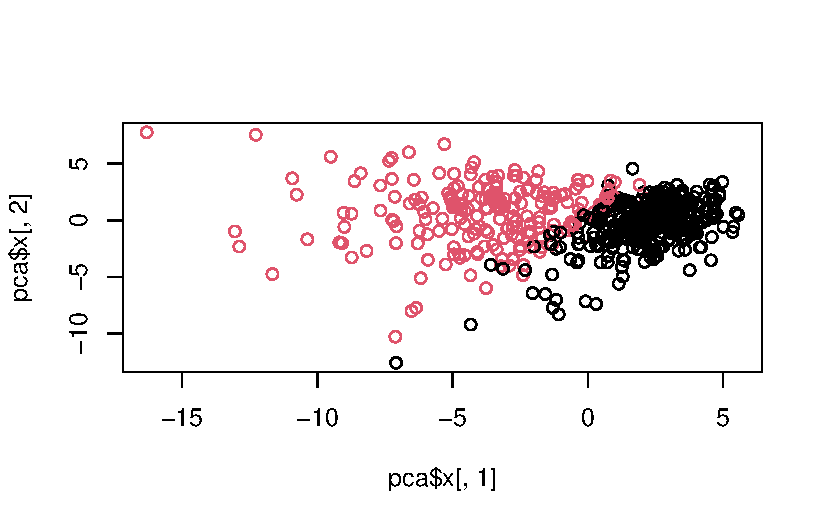
\includegraphics{class08_files/figure-pdf/unnamed-chunk-10-1.pdf}

}

\end{figure}

Plot PC2 against PC1 with ggplot.

\begin{Shaded}
\begin{Highlighting}[]
\FunctionTok{library}\NormalTok{(ggplot2)}

\FunctionTok{ggplot}\NormalTok{(}\FunctionTok{as.data.frame}\NormalTok{(pca}\SpecialCharTok{$}\NormalTok{x)) }\SpecialCharTok{+}
  \FunctionTok{aes}\NormalTok{(PC1,PC2,}\AttributeTok{col=}\NormalTok{diagnosis) }\SpecialCharTok{+}
  \FunctionTok{geom\_point}\NormalTok{()}
\end{Highlighting}
\end{Shaded}

\begin{figure}[H]

{\centering 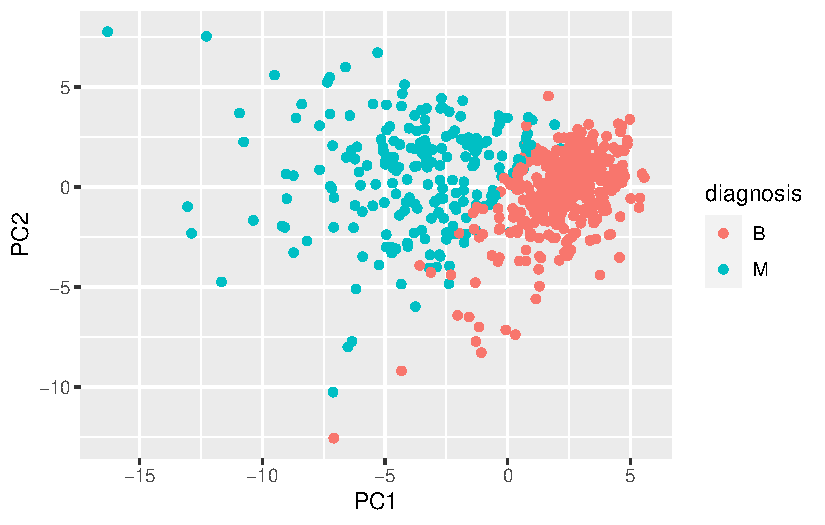
\includegraphics{class08_files/figure-pdf/unnamed-chunk-11-1.pdf}

}

\end{figure}

\begin{quote}
Q. How much variance is captured in the top 3 PCs.
\end{quote}

They capture 76.636\% of total variance.

rotation is the influence of each of the original \textbf{variables}
upon the principal components (typically known as loading scores)

\begin{quote}
Q9. For the first principal component, what is the component of the
loading vector (i.e.~wisc.pr\$rotation{[},1{]}) for the feature
concave.points\_mean? This tells us how much this original feature
contributes to the first PC.
\end{quote}

\begin{Shaded}
\begin{Highlighting}[]
\NormalTok{pca}\SpecialCharTok{$}\NormalTok{rotation[}\StringTok{"concave.points\_mean"}\NormalTok{,}\DecValTok{1}\NormalTok{]}
\end{Highlighting}
\end{Shaded}

\begin{verbatim}
[1] -0.2608538
\end{verbatim}

\hypertarget{combine-pca-results-with-clustering}{%
\section{Combine PCA results with
clustering}\label{combine-pca-results-with-clustering}}

We can use new PCA variables (i.e.~the scores along the PCs contained in
\texttt{pca\$x}) as input for other methods such as clustering.

\begin{Shaded}
\begin{Highlighting}[]
\CommentTok{\#hclust need distance matrix as input}
\NormalTok{d }\OtherTok{\textless{}{-}} \FunctionTok{dist}\NormalTok{(pca}\SpecialCharTok{$}\NormalTok{x[,}\DecValTok{1}\SpecialCharTok{:}\DecValTok{3}\NormalTok{])}
\NormalTok{hc }\OtherTok{\textless{}{-}} \FunctionTok{hclust}\NormalTok{(d, }\AttributeTok{method=}\StringTok{"ward.D2"}\NormalTok{)}
\FunctionTok{plot}\NormalTok{(hc)}
\end{Highlighting}
\end{Shaded}

\begin{figure}[H]

{\centering 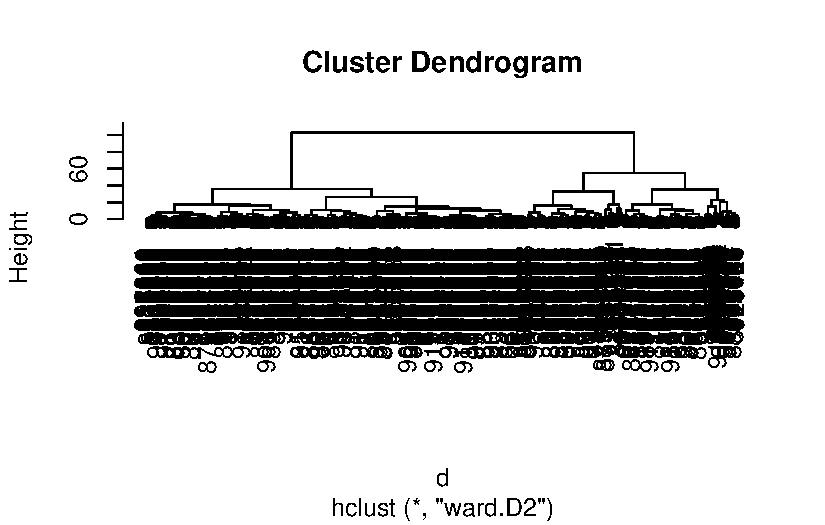
\includegraphics{class08_files/figure-pdf/unnamed-chunk-13-1.pdf}

}

\end{figure}

To get our cluster membership vector we can use the \texttt{cutree()}
function and specify a height(\texttt{h}) or numbder of groups
(\texttt{k}) in arguments.

\begin{Shaded}
\begin{Highlighting}[]
\NormalTok{grps }\OtherTok{\textless{}{-}} \FunctionTok{cutree}\NormalTok{(hc,}\AttributeTok{k=}\DecValTok{2}\NormalTok{)}
\FunctionTok{table}\NormalTok{(grps)}
\end{Highlighting}
\end{Shaded}

\begin{verbatim}
grps
  1   2 
203 366 
\end{verbatim}

I want to find out how many benign(``B'') and malignant(``M'') are in
each group

\begin{Shaded}
\begin{Highlighting}[]
\FunctionTok{table}\NormalTok{(diagnosis,grps)}
\end{Highlighting}
\end{Shaded}

\begin{verbatim}
         grps
diagnosis   1   2
        B  24 333
        M 179  33
\end{verbatim}

We can also make a plot using clustering factor \texttt{grps}

\begin{Shaded}
\begin{Highlighting}[]
\FunctionTok{ggplot}\NormalTok{(}\FunctionTok{as.data.frame}\NormalTok{(pca}\SpecialCharTok{$}\NormalTok{x)) }\SpecialCharTok{+}
  \FunctionTok{aes}\NormalTok{(PC1,PC2,}\AttributeTok{col=}\FunctionTok{factor}\NormalTok{(grps)) }\SpecialCharTok{+}
  \FunctionTok{geom\_point}\NormalTok{()}
\end{Highlighting}
\end{Shaded}

\begin{figure}[H]

{\centering 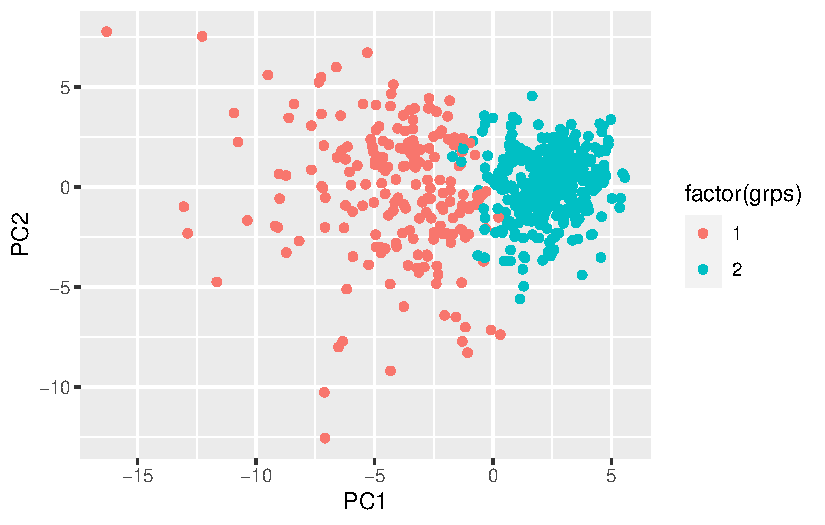
\includegraphics{class08_files/figure-pdf/unnamed-chunk-16-1.pdf}

}

\end{figure}

\begin{quote}
Q15. OPTIONAL: Which of your analysis procedures resulted in a
clustering model with the best specificity? How about sensitivity?
\end{quote}

\textbf{Sensitivity} refers to a test's ability to correctly detect ill
patients who do have the condition. In our example here the sensitivity
is the total number of samples in the cluster identified as
predominantly malignant (cancerous) divided by the total number of known
malignant samples. In other words: TP/(TP+FN).

\textbf{Specificity} relates to a test's ability to correctly reject
healthy patients without a condition. In our example specificity is the
proportion of benign (not cancerous) samples in the cluster identified
as predominantly benign that are known to be benign. In other words:
TN/(TN+FN).

\begin{Shaded}
\begin{Highlighting}[]
\DecValTok{179}\SpecialCharTok{/}\NormalTok{(}\DecValTok{179}\SpecialCharTok{+}\DecValTok{33}\NormalTok{)}
\end{Highlighting}
\end{Shaded}

\begin{verbatim}
[1] 0.8443396
\end{verbatim}

\begin{Shaded}
\begin{Highlighting}[]
\DecValTok{333}\SpecialCharTok{/}\NormalTok{(}\DecValTok{333}\SpecialCharTok{+}\DecValTok{24}\NormalTok{)}
\end{Highlighting}
\end{Shaded}

\begin{verbatim}
[1] 0.9327731
\end{verbatim}

Sensitivity = TP/(TP+FN) = 179/(179+33) = 0.8443396

Specificity = TN/(TN+FN) = 333/(333+24) = 0.9327731

\hypertarget{prediction}{%
\section{Prediction}\label{prediction}}

\begin{Shaded}
\begin{Highlighting}[]
\NormalTok{url }\OtherTok{\textless{}{-}} \StringTok{"https://tinyurl.com/new{-}samples{-}CSV"}
\NormalTok{new }\OtherTok{\textless{}{-}} \FunctionTok{read.csv}\NormalTok{(url)}
\NormalTok{npc }\OtherTok{\textless{}{-}} \FunctionTok{predict}\NormalTok{(pca, }\AttributeTok{newdata=}\NormalTok{new)}
\NormalTok{npc}
\end{Highlighting}
\end{Shaded}

\begin{verbatim}
           PC1       PC2        PC3        PC4       PC5        PC6        PC7
[1,]  2.576616 -3.135913  1.3990492 -0.7631950  2.781648 -0.8150185 -0.3959098
[2,] -4.754928 -3.009033 -0.1660946 -0.6052952 -1.140698 -1.2189945  0.8193031
            PC8       PC9       PC10      PC11      PC12      PC13     PC14
[1,] -0.2307350 0.1029569 -0.9272861 0.3411457  0.375921 0.1610764 1.187882
[2,] -0.3307423 0.5281896 -0.4855301 0.7173233 -1.185917 0.5893856 0.303029
          PC15       PC16        PC17        PC18        PC19       PC20
[1,] 0.3216974 -0.1743616 -0.07875393 -0.11207028 -0.08802955 -0.2495216
[2,] 0.1299153  0.1448061 -0.40509706  0.06565549  0.25591230 -0.4289500
           PC21       PC22       PC23       PC24        PC25         PC26
[1,]  0.1228233 0.09358453 0.08347651  0.1223396  0.02124121  0.078884581
[2,] -0.1224776 0.01732146 0.06316631 -0.2338618 -0.20755948 -0.009833238
             PC27        PC28         PC29         PC30
[1,]  0.220199544 -0.02946023 -0.015620933  0.005269029
[2,] -0.001134152  0.09638361  0.002795349 -0.019015820
\end{verbatim}

\begin{Shaded}
\begin{Highlighting}[]
\FunctionTok{plot}\NormalTok{(pca}\SpecialCharTok{$}\NormalTok{x[,}\DecValTok{1}\SpecialCharTok{:}\DecValTok{2}\NormalTok{],}\AttributeTok{col=}\NormalTok{grps)}
\FunctionTok{points}\NormalTok{(npc[,}\DecValTok{1}\NormalTok{], npc[,}\DecValTok{2}\NormalTok{], }\AttributeTok{col=}\StringTok{"blue"}\NormalTok{, }\AttributeTok{pch=}\DecValTok{16}\NormalTok{, }\AttributeTok{cex=}\DecValTok{3}\NormalTok{)}
\FunctionTok{text}\NormalTok{(npc[,}\DecValTok{1}\NormalTok{], npc[,}\DecValTok{2}\NormalTok{], }\FunctionTok{c}\NormalTok{(}\DecValTok{1}\NormalTok{,}\DecValTok{2}\NormalTok{), }\AttributeTok{col=}\StringTok{"white"}\NormalTok{)}
\end{Highlighting}
\end{Shaded}

\begin{figure}[H]

{\centering 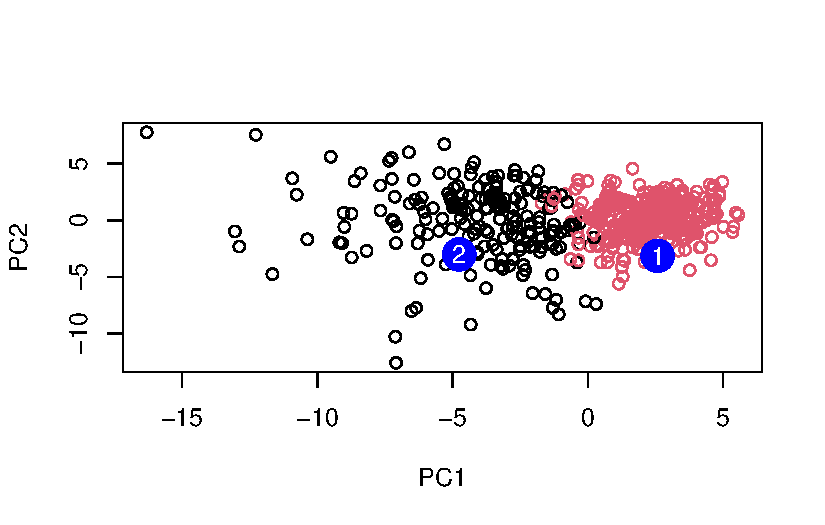
\includegraphics{class08_files/figure-pdf/unnamed-chunk-19-1.pdf}

}

\end{figure}

\begin{quote}
Q16. Which of these new patients should we prioritize for follow up
based on your results?
\end{quote}

We should prioritize patient 2. Patient 2's position on the plot is in
the clustering of group 1 in \texttt{grps}, in which most of them have
malignant tumor. Meanwhile, patient 1's position on the plot is in the
clustering of group 2 in \texttt{grps}, in which most of them have
benign tumor.



\end{document}
